\documentclass[11pt]{article}
\usepackage[margin=0.75in]{geometry}
\usepackage[T1]{fontenc}
\usepackage{helvet}
\renewcommand{\familydefault}{\sfdefault}
\usepackage{tikz}
\usetikzlibrary{decorations.pathreplacing}
\usepackage{array}
\usepackage{enumitem}
\pagestyle{empty}
\setlength{\parindent}{0pt}
\setlist[enumerate,2]{label=(\alph*),leftmargin=2em,itemsep=2.2em}

% Build the key with:  pdflatex -jobname=<name>_KEY "\def\iskey{}\input{<name>}"
\newif\ifkey
\ifdefined\iskey \keytrue \fi
\newcommand{\ans}[1]{\ifkey\leavevmode{\color{red!75!black}#1}\fi}

% ---------- helpers ----------
% number line: \nline{min}{max}{label step}{axis label}   (1 unit = \xu)
\newcommand{\nline}[4]{%
  \draw[thick] (#1-0.5,0) -- (#2+0.5,0);
  \foreach \t in {#1,...,#2} \draw (\t,0.12) -- (\t,-0.12);
  \pgfmathtruncatemacro{\nxt}{#1+#3}
  \foreach \t in {#1,\nxt,...,#2} \draw (\t,0.2) -- (\t,-0.2) node[below] {\t};
  \node at ({(#1+#2)/2},-0.95) {#4};}
% box plot above the line: \bplot{min}{Q1}{med}{Q3}{max}
\newcommand{\bplot}[5]{%
  \draw[thick] (#1,1.0) -- (#2,1.0);
  \draw[thick] (#4,1.0) -- (#5,1.0);
  \draw[thick] (#1,0.75) -- (#1,1.25);
  \draw[thick] (#5,0.75) -- (#5,1.25);
  \draw[thick,fill=gray!20] (#2,0.55) rectangle (#4,1.45);
  \draw[very thick] (#3,0.55) -- (#3,1.45);}
% dot plot: \dotplot{min}{max}{value/count,...}{axis label}
\newcommand{\dotplot}[4]{%
\begin{tikzpicture}[x=0.9cm,y=0.33cm]
  \draw[thick] (#1-0.5,0) -- (#2+0.5,0);
  \foreach \t in {#1,...,#2} {\draw (\t,0.25) -- (\t,-0.25) node[below] {\t};}
  \foreach \v/\c in {#3} {\ifnum\c>0 \foreach \k in {1,...,\c} {\fill (\v,\k*1.15) circle (0.16cm);}\fi}
  \node at ({(#1+#2)/2},-2.3) {#4};
\end{tikzpicture}}

\begin{document}

{\Large\bfseries Quartiles, IQR, and Box Plots\ifkey\ \textcolor{red!75!black}{KEY}\fi}\hfill Name \underline{\hspace{2in}}

\vspace{0.6em}
Quartiles cut the data into \textbf{4 equal parts}. Each part has about \textbf{25\%} of the data.

\vspace{0.6em}
\renewcommand{\arraystretch}{1.3}
\begin{tabular}{|>{\raggedright}p{3.25in}|>{\raggedright\arraybackslash}p{3.25in}|}
\hline
\textbf{How to find the quartiles} & \textbf{Five-number summary} \\
1. Put the data in order.\newline
2. Find the \textbf{median}. It splits the data into a \textbf{lower half} and an \textbf{upper half}.\newline
3. \textbf{Q1} = median of the lower half.\newline
4. \textbf{Q3} = median of the upper half.\newline
\textbf{Odd number of values?} Leave the median out of both halves. &
Minimum\newline Q1\newline Median\newline Q3\newline Maximum\par\vspace{0.4em}
\textbf{IQR = Q3 $-$ Q1}\newline
The IQR (interquartile range) is how spread out the \textbf{middle half} of the data is. \\
\hline
\end{tabular}

\vspace{0.9em}
\textbf{Example 1: odd number of values (11)}

\vspace{0.3em}
\begin{tabular}{@{}l}
3,\; 4,\; 6,\; 7,\; 9,\; \fbox{10},\; 12,\; 13,\; 15,\; 18,\; 20 \qquad Median = 10 (leave it out of the halves)\\[0.3em]
Lower half: 3,\; 4,\; \fbox{6},\; 7,\; 9 \;\;$\rightarrow$\;\; Q1 = 6 \qquad
Upper half: 12,\; 13,\; \fbox{15},\; 18,\; 20 \;\;$\rightarrow$\;\; Q3 = 15\\[0.3em]
IQR = 15 $-$ 6 = \textbf{9}
\end{tabular}

\vspace{0.8em}
\textbf{Example 2: even number of values (10)}

\vspace{0.3em}
\begin{tabular}{@{}l}
1,\; 3,\; 4,\; 6,\; \fbox{7},\; \fbox{9},\; 10,\; 12,\; 14,\; 18 \qquad Median = (7 + 9) $\div$ 2 = 8\\[0.3em]
Lower half: 1,\; 3,\; \fbox{4},\; 6,\; 7 \;\;$\rightarrow$\;\; Q1 = 4 \qquad
Upper half: 9,\; 10,\; \fbox{12},\; 14,\; 18 \;\;$\rightarrow$\;\; Q3 = 12\\[0.3em]
IQR = 12 $-$ 4 = \textbf{8}
\end{tabular}

\vspace{0.9em}
\textbf{A box plot draws the five-number summary.} Here is Example 1.

\begin{center}
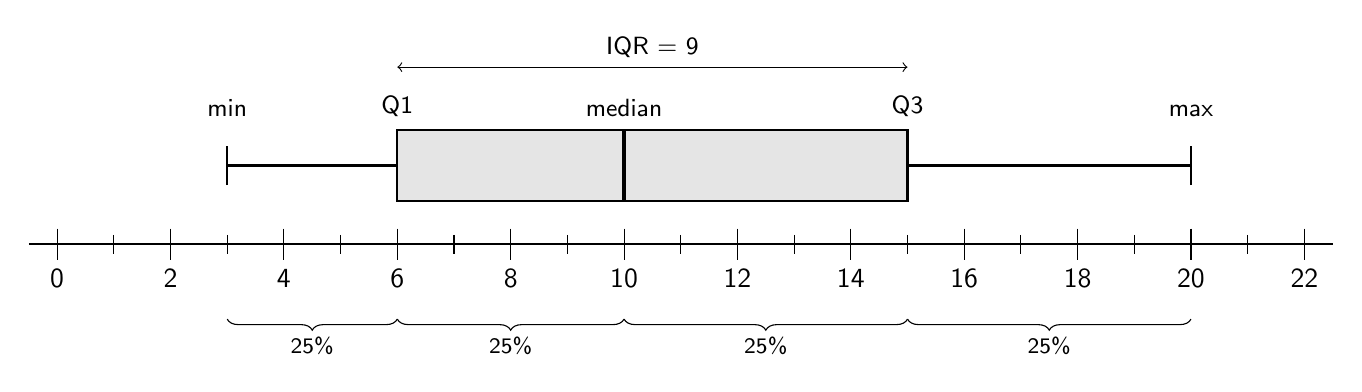
\begin{tikzpicture}[x=0.72cm,y=1cm]
  \nline{0}{22}{2}{}
  \bplot{3}{6}{10}{15}{20}
  \foreach \x/\l in {3/min,6/Q1,10/median,15/Q3,20/max}
    \node[font=\small,above] at (\x,1.5) {\l};
  \foreach \a/\b in {3/6,6/10,10/15,15/20}
    \draw[decorate,decoration={brace,amplitude=4pt,mirror}] (\a,-0.95) -- (\b,-0.95)
      node[midway,below=3pt,font=\footnotesize] {25\%};
  \draw[<->] (6,2.25) -- (15,2.25) node[midway,above,font=\small] {IQR = 9};
\end{tikzpicture}
\end{center}

\textbf{Gotcha:} The 4 parts have the same \textbf{number of values}, not the same width.
A short part means the values are packed close together.

\vspace{0.4em}
Work with a partner. Compare answers when you finish each problem.

% ---------------- PROBLEMS ----------------
\newpage
\begin{enumerate}[leftmargin=1.5em,itemsep=1em]

\item Find the five-number summary and the IQR.
\begin{center}4,\; 8,\; 1,\; 6,\; 9,\; 3,\; 7\end{center}
\ans{In order: 1, 3, 4, \fbox{6}, 7, 8, 9. \quad Min 1, Q1 3, Median 6, Q3 8, Max 9. \quad IQR = 8 $-$ 3 = 5}
\vspace{6em}

\item Find the five-number summary and the IQR.
\begin{center}12,\; 15,\; 10,\; 20,\; 18,\; 11,\; 16,\; 14\end{center}
\ans{In order: 10, 11, 12, 14, 15, 16, 18, 20. \quad Median = (14 + 15) $\div$ 2 = 14.5\\
Lower half 10, 11, 12, 14: Q1 = 11.5. \quad Upper half 15, 16, 18, 20: Q3 = 17.\\
Min 10, Q1 11.5, Median 14.5, Q3 17, Max 20. \quad IQR = 5.5}
\vspace{6em}

\item Eleven students recorded how many minutes they spent on homework last night.
\begin{center}30,\; 10,\; 45,\; 5,\; 25,\; 60,\; 15,\; 30,\; 10,\; 40,\; 20\end{center}
\begin{enumerate}[itemsep=1em]
  \item Find the five-number summary.

  \ans{5, 10, 10, 15, 20, \fbox{25}, 30, 30, 40, 45, 60. \quad Min 5, Q1 10, Median 25, Q3 40, Max 60}
  \vspace{5em}
  \item Make a box plot.
  \begin{center}
  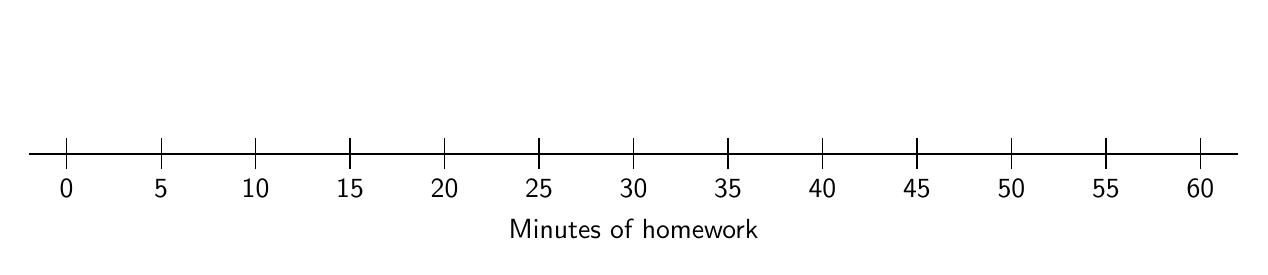
\begin{tikzpicture}[x=0.24cm,y=1cm]
    \draw[thick] (-2,0) -- (62,0);
    \foreach \t in {0,5,...,60} \draw (\t,0.2) -- (\t,-0.2) node[below] {\t};
    \node at (30,-0.95) {Minutes of homework};
    \ifkey\begin{scope}[red!75!black]\bplot{5}{10}{25}{40}{60}\end{scope}\else\path (0,1.6);\fi
  \end{tikzpicture}
  \end{center}
  \item What is the IQR? What does it tell you?

  \ans{40 $-$ 10 = 30 minutes. The middle half of the students spent between 10 and 40 minutes, a spread of 30 minutes.}
\end{enumerate}

\newpage
\item Twelve students counted how many texts they sent in one hour.
\begin{center}13,\; 2,\; 20,\; 8,\; 30,\; 12,\; 5,\; 18,\; 10,\; 24,\; 8,\; 15\end{center}
\begin{enumerate}[itemsep=1em]
  \item Find the five-number summary.

  \ans{2, 5, 8, 8, 10, \fbox{12}, \fbox{13}, 15, 18, 20, 24, 30. \quad Median 12.5\\
  Lower half 2, 5, 8, 8, 10, 12: Q1 = 8. \quad Upper half 13, 15, 18, 20, 24, 30: Q3 = 19.\\
  Min 2, Q1 8, Median 12.5, Q3 19, Max 30}
  \vspace{5em}
  \item Make a box plot.
  \begin{center}
  \begin{tikzpicture}[x=0.48cm,y=1cm]
    \nline{0}{30}{5}{Texts sent in one hour}
    \ifkey\begin{scope}[red!75!black]\bplot{2}{8}{12.5}{19}{30}\end{scope}\else\path (0,1.6);\fi
  \end{tikzpicture}
  \end{center}
  \item Which part of the box plot is the longest? What does that tell you about the data?

  \ans{The right whisker (19 to 30). The top 25\% of students are spread out the most.}
\end{enumerate}
\vspace{1.5em}

\item This dot plot shows how many pets some students have.
\begin{center}\dotplot{1}{8}{1/2,2/3,3/4,4/3,5/2,6/1,7/0,8/1}{Number of pets}\end{center}
\begin{enumerate}
  \item How many students are in the data?
  \ans{\quad 16}
  \item Find Q1, the median, and Q3.

  \ans{1, 1, 2, 2, 2, 3, 3, \fbox{3}, \fbox{3}, 4, 4, 4, 5, 5, 6, 8. \quad Median 3\\
  Lower half: 1, 1, 2, 2, 2, 3, 3, 3 \;$\rightarrow$\; Q1 = 2. \quad Upper half: 3, 4, 4, 4, 5, 5, 6, 8 \;$\rightarrow$\; Q3 = 4.5}
  \vspace{2em}
  \item Find the IQR.
  \ans{\quad 4.5 $-$ 2 = 2.5}
\end{enumerate}

\newpage
\item Look at these two data sets.
\begin{center}
\renewcommand{\arraystretch}{1.4}
\begin{tabular}{ll}
Set A: & 1,\; 2,\; 3,\; 4,\; 5,\; 6,\; 7 \\
Set B: & 1,\; 2,\; 3,\; 4,\; 5,\; 6,\; 70
\end{tabular}
\end{center}
\begin{enumerate}
  \item Find the IQR of each set.

  \ans{Both: Q1 = 2, Q3 = 6, IQR = 4}
  \vspace{2em}
  \item Find the range (max $-$ min) of each set.

  \ans{A: 7 $-$ 1 = 6. \quad B: 70 $-$ 1 = 69}
  \vspace{2em}
  \item One number changed. Which measure of spread changed a lot? Which did not change? Why?

  \ans{The range changed a lot. The IQR did not change. The IQR only uses the middle half, so one extreme value does not move it. This is like the median vs the mean.}
\end{enumerate}

\end{enumerate}

\end{document}
